\documentclass[10pt,a4paper]{article}
\usepackage[utf8]{inputenc}
\usepackage[spanish]{babel}
\usepackage{amsmath}
\usepackage{amsfonts}
\usepackage{amssymb}
\usepackage{graphicx}
\usepackage{subfig}
\renewcommand{\contentsname}{Contenidos}
\renewcommand{\abstractname}{Resumen}
\renewcommand{\refname}{Referencias}

\begin{document}
\title{La Gramola \\\normalsize Proyecto de aplicación para Curso Android 2015-2016}
\author{
	Estévez Casado, Fernando\\
	\texttt{fernando0estevez@gmail.com}
	\and 
	Laso Rodríguez, Rubén
	\\
	\texttt{ruben.laso.rguez@gmail.com}\\
\\Universidade de Santiago de Compostela, Galicia}
\date{Domingo, 14 de febrero de 2016}
\maketitle

\begin{abstract}
La Gramola es un reproductor de archivos de audio que te permitirá aprender las letras de las canciones que tengas en tu dispositivo, mostrándotelas cómodamente en la pantalla al mismo tiempo que se reproducen.
\end{abstract}

\tableofcontents
\newpage
\renewcommand{\abstractname}{Resumen}
\renewcommand{\tablename}{Tabla}
\renewcommand{\figurename}{Figura}

\section{Introducción}
La Gramola es un reproductor de archivos de audio. Este muestra los archivos \texttt{.mp3} que tenemos en nuestro dispositivo en una lista ordenada por autor, como se puede ver en la Figura \ref{fig:lista}. En dicha lista se muestra el título de cada canción, así como su autor y el álbum al que pertenece. 

\begin{figure}[htbp]
	\centering
		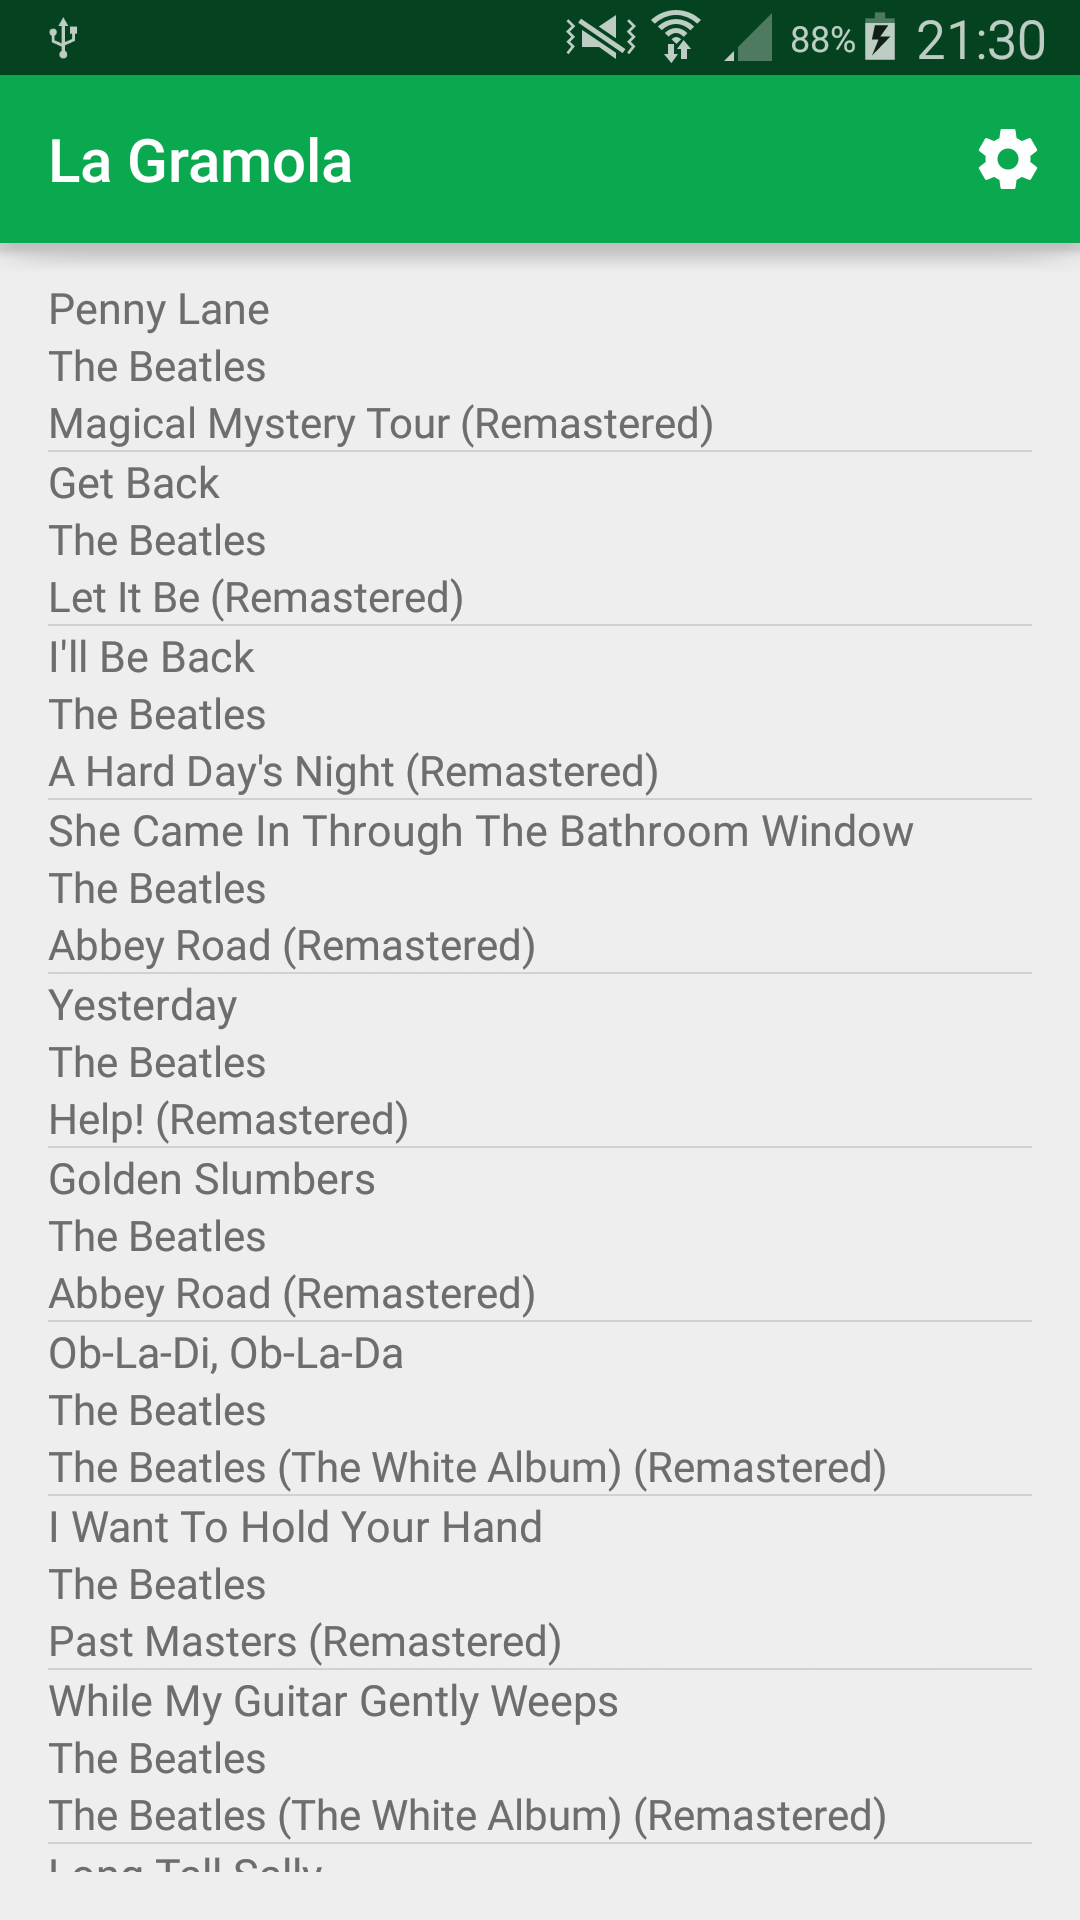
\includegraphics[width=0.5\textwidth]{capturas/lista.png}
	\caption{Captura de pantalla de la \texttt{MainActivity}, mostrando la lista de archivos de audio.}
	\label{fig:lista}
\end{figure}

\section{Funcionamiento básico}
Pulsando sobre cualquier entrada se nos abrirá el reproductor y automáticamente comenzará a sonar la canción escogida, como se puede ver en la Figura \ref{fig:playerVertical}. Podremos pausar, reanudar, avanzar y retroceder en el audio con los botones universales que se proporcionan. A mayores, podremos avanzar a la siguiente canción o retroceder a la anterior.\\

El primer botón de la parte superior activará el modo aleatorio, con el cual el orden de las canciones será totalmente aleatorio.\\

La nota musical (el segundo de los iconos superiores) mostrará la letra de la canción en caso de que la app la pueda encontrar (ver Figura \ref{fig:playerVerticalLyrics}). En otro caso mostrará un mensaje de error. \\El mecanismo para encontrar las letras es simple. Se toman los datos de la pista (título y autor) y se realiza una consulta a la API de Musixmatch. Primero se busca la pista en su base de datos con la información de la que disponemos. Si conseguimos obtener una coincidencia, usamos el ID que se nos devuelve para obtener los \textit{lyrics}.\\

\begin{figure}[htbp]
	\centering
          \subfloat[Vista vertical del reproductor.]{
           \label{fig:playerVertical}
            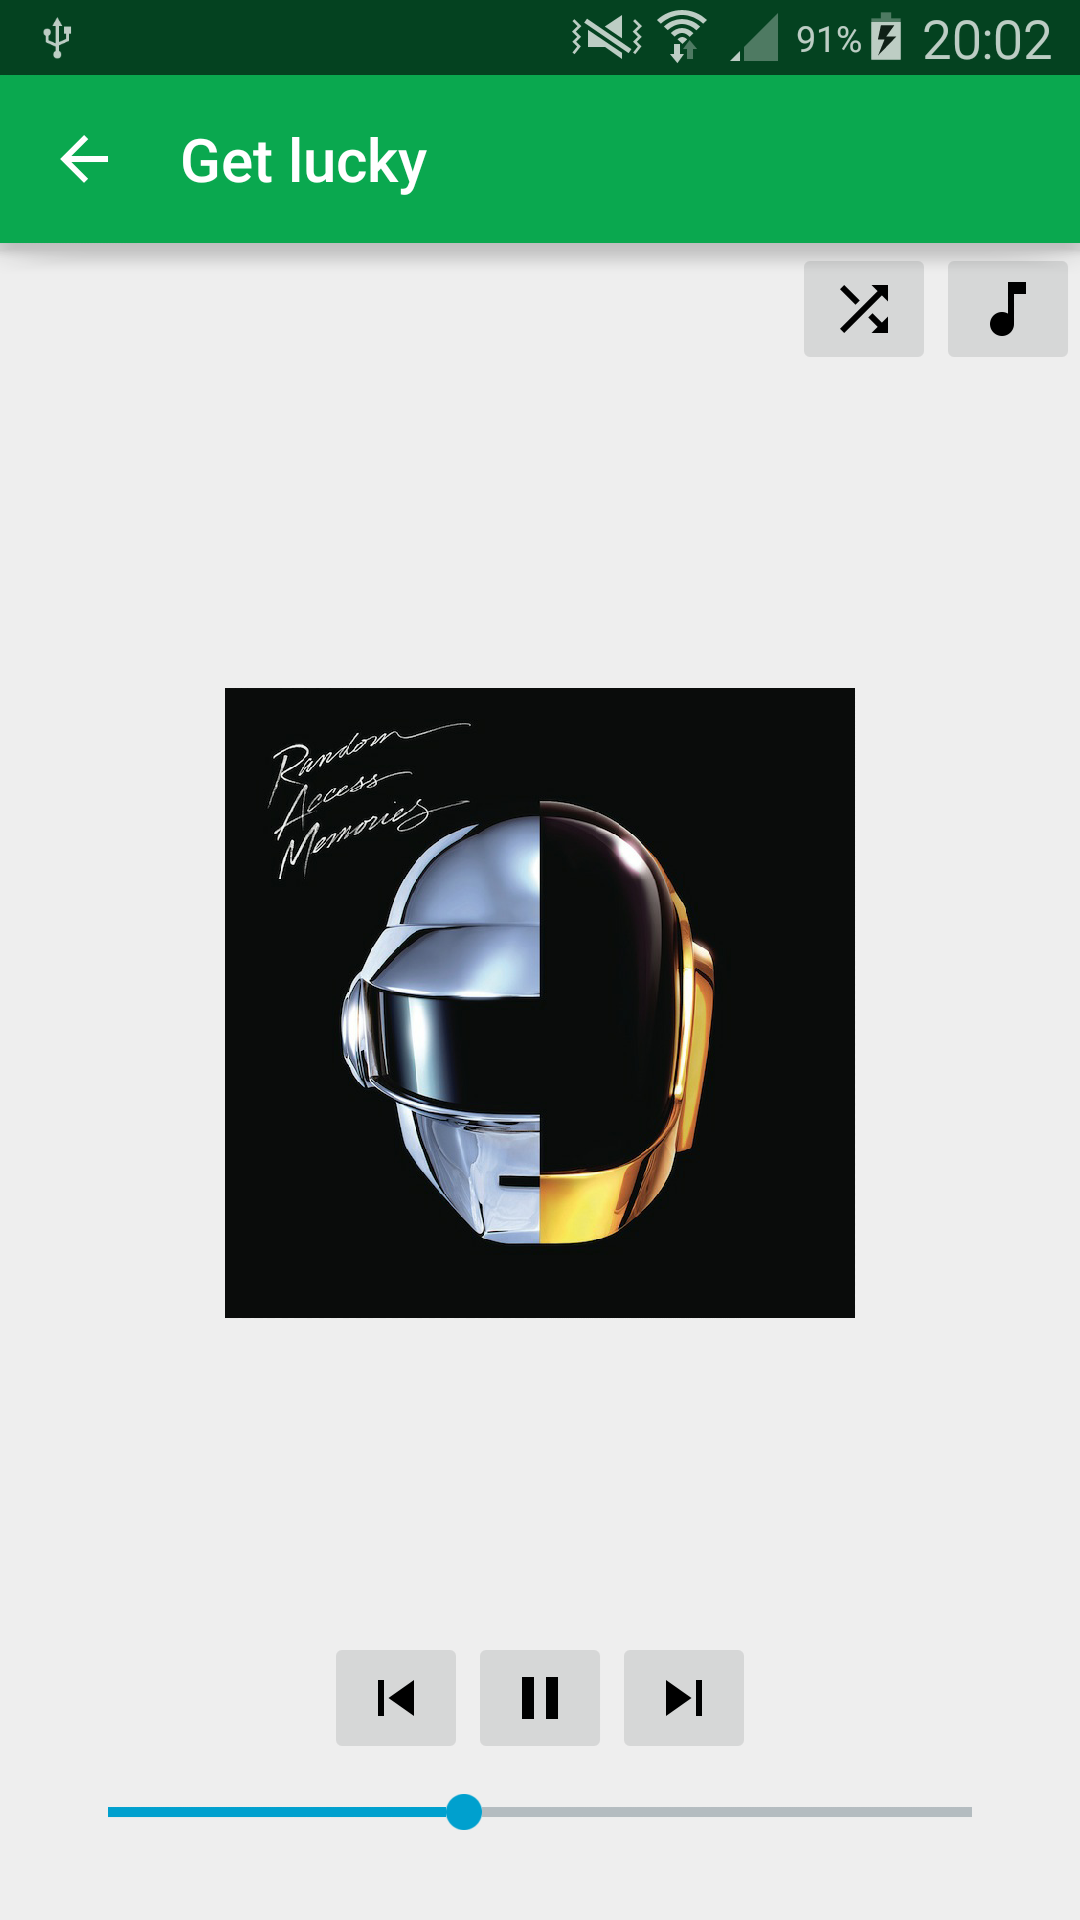
\includegraphics[width=0.5\textwidth]{capturas/playerVertical.png}}
	    \subfloat[Vista vertical con la letra de la canción.]{
           \label{fig:playerVerticalLyrics}
		   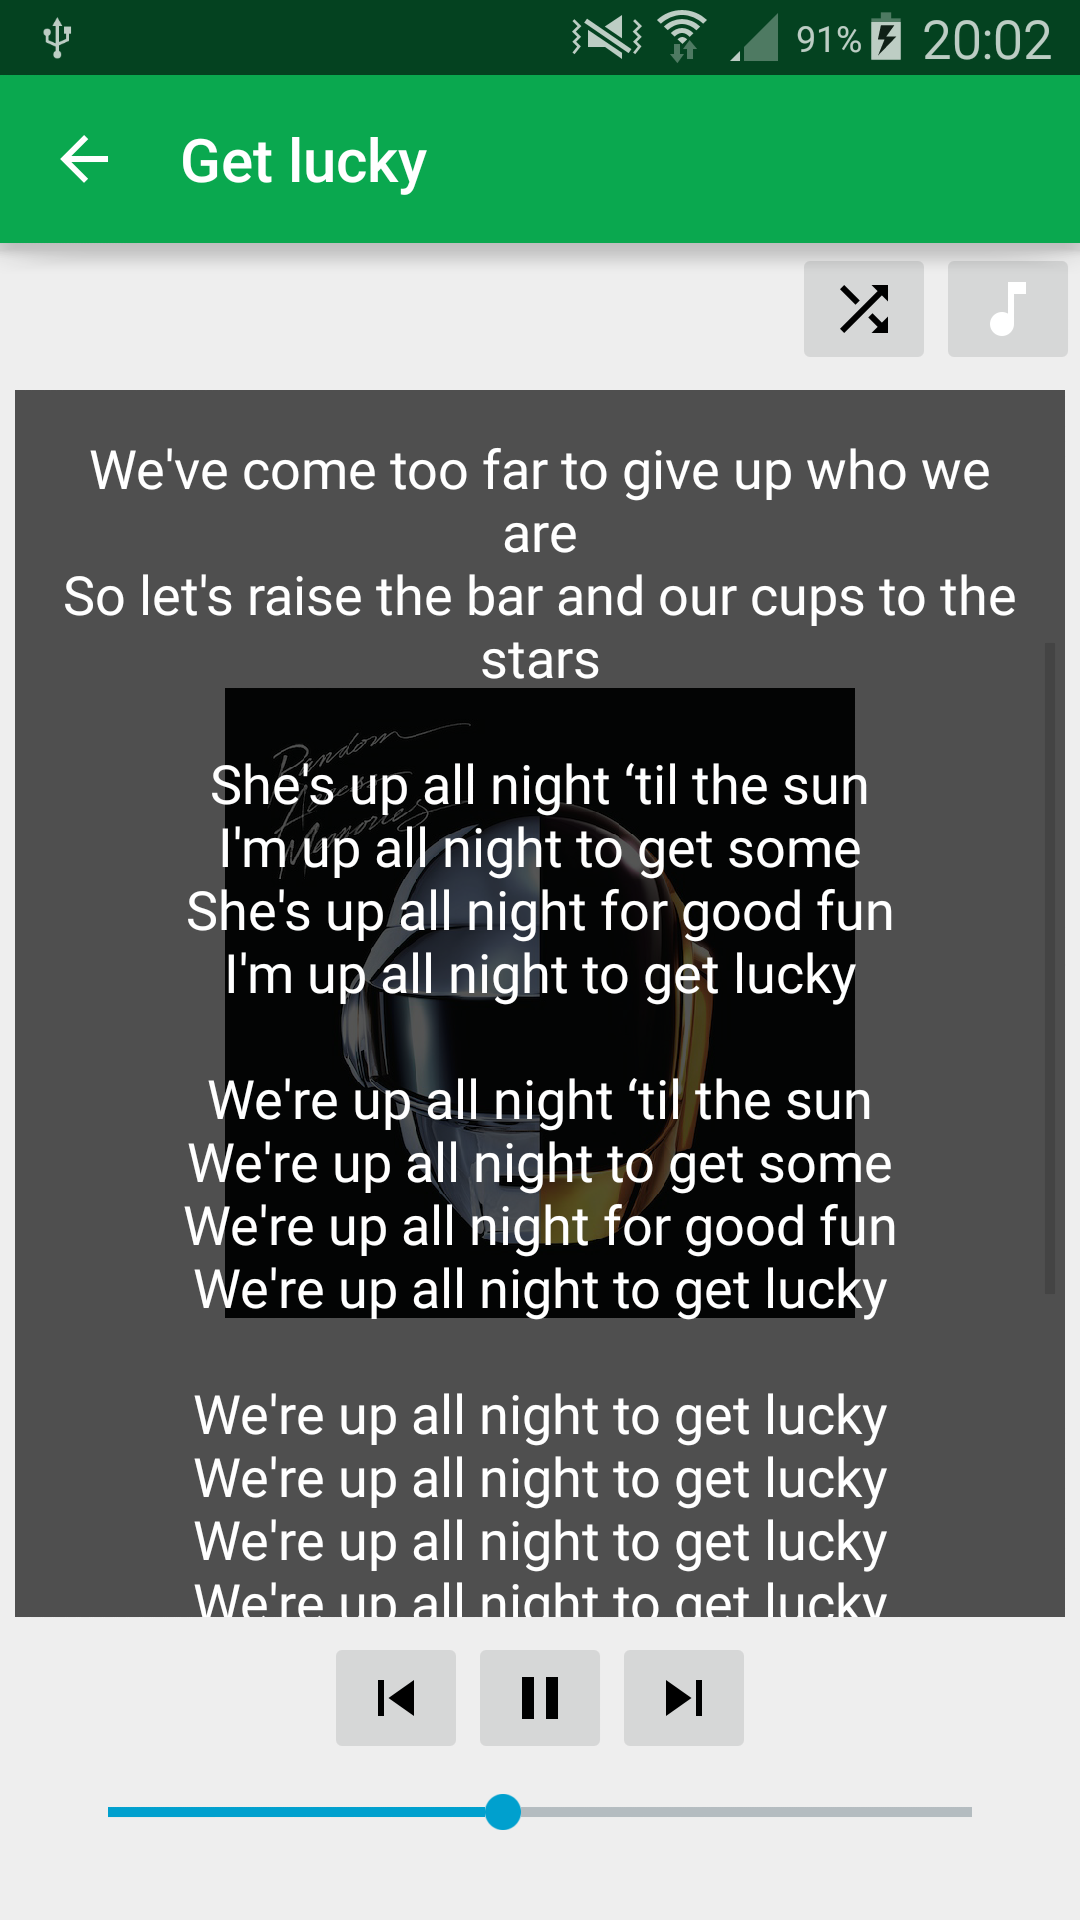
\includegraphics[width=0.5\textwidth]{capturas/playerVerticalLyrics.png}}
	\caption{Vistas verticales del reproductor}
	\label{fig:vertical}
\end{figure}

El reproductor dispone de una vista vertical (Figuras \ref{fig:playerVertical} y \ref{fig:playerVerticalLyrics}) y otra apaisada (Figuras \ref{fig:horizontal} y \ref{fig:horizontal_lyrics}). Cada una de ellas optimiza la disposición de la información mostrada por pantalla.\\


\begin{figure}[htbp]
	\centering
		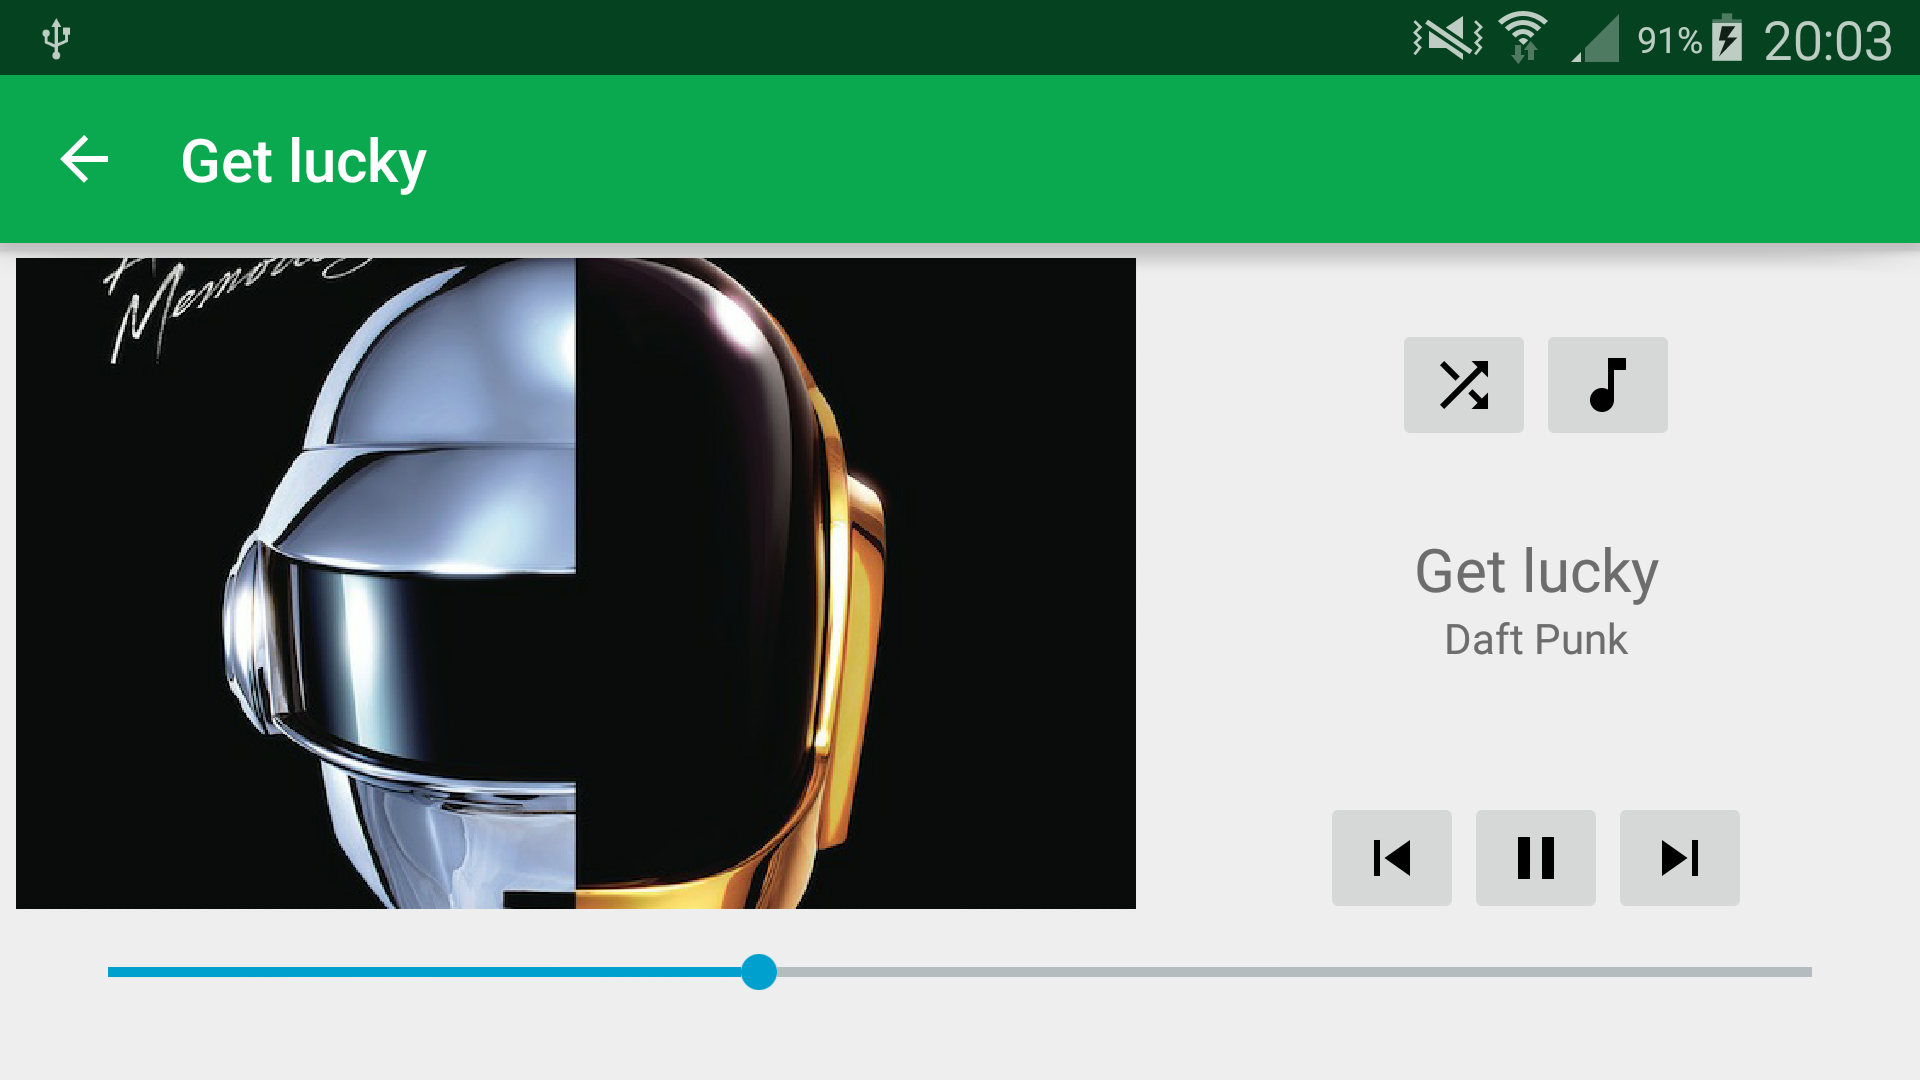
\includegraphics[width=0.8\textwidth]{capturas/PlayerHorizontal.png}
	\caption{Captura de pantalla de la \texttt{PlayerActivity} (vista apaisada).}
	\label{fig:horizontal}
\end{figure}

\begin{figure}[htbp]
	\centering
		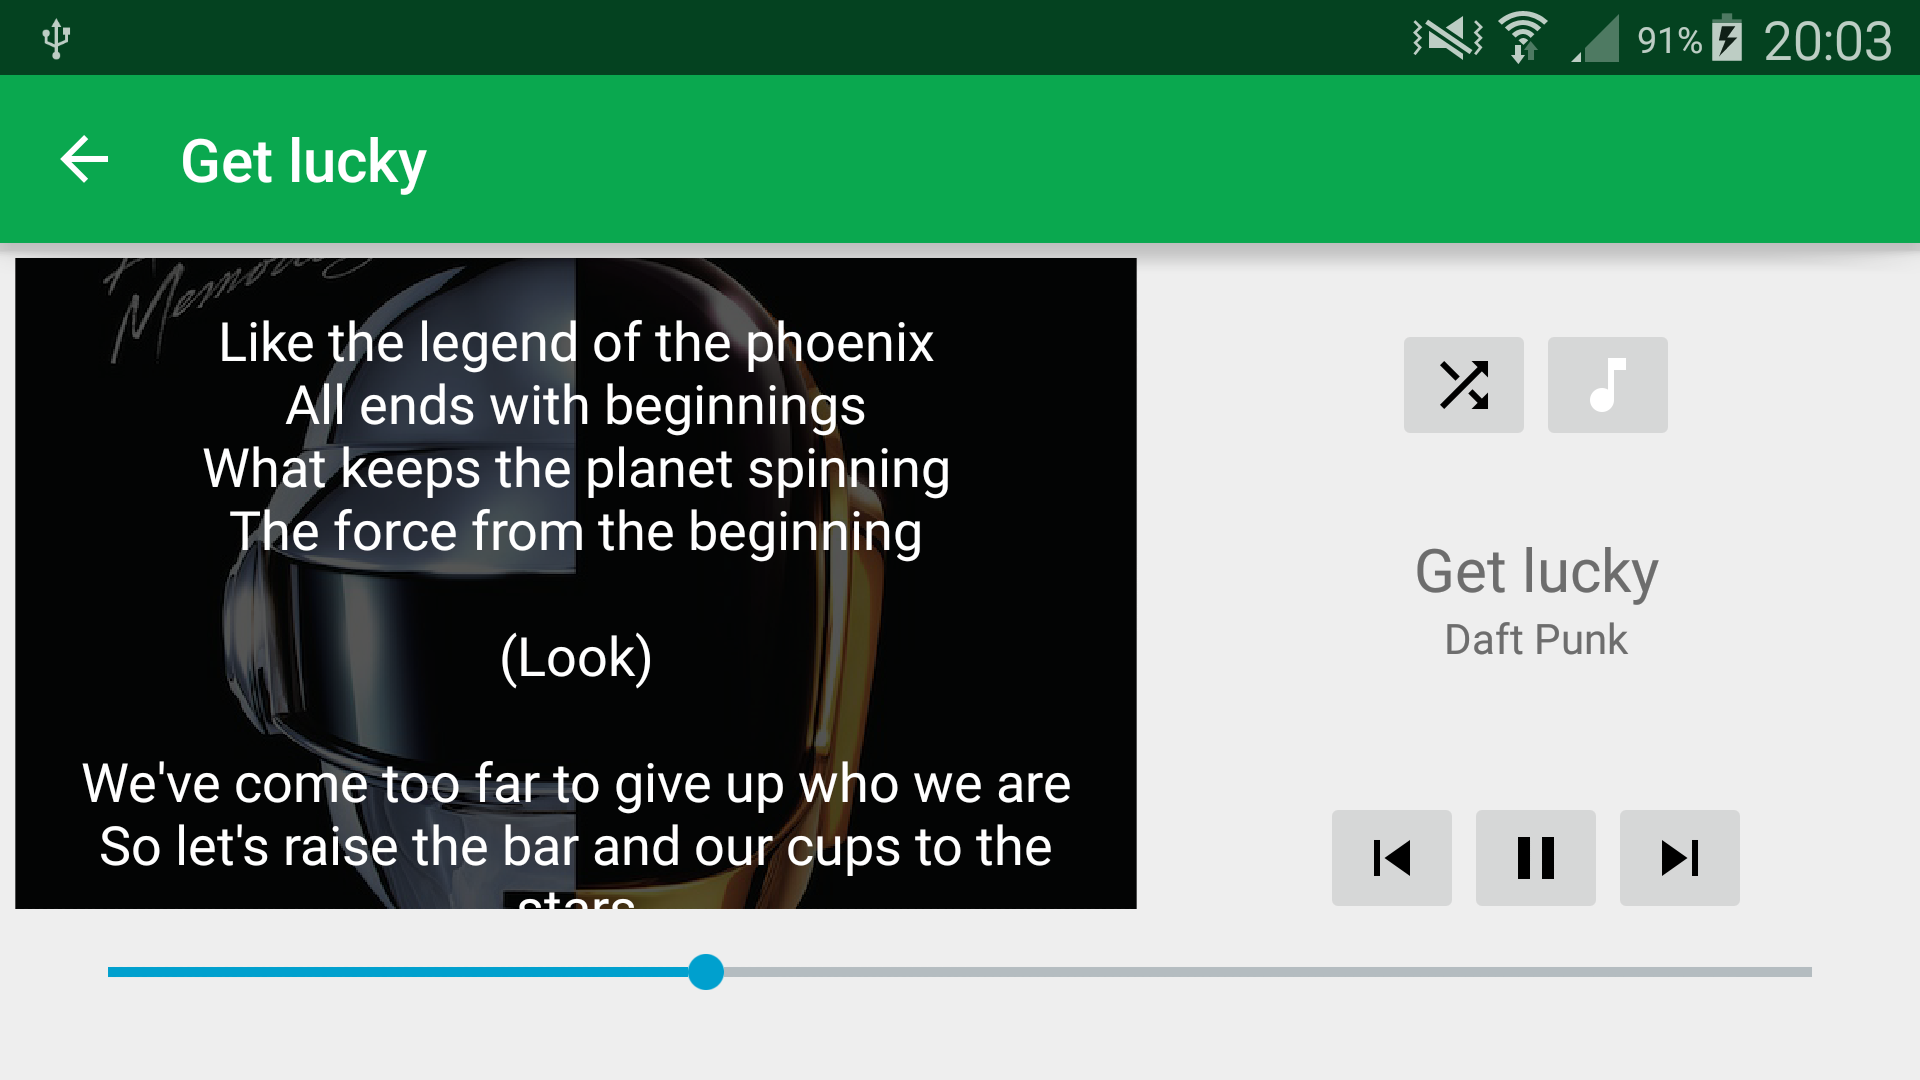
\includegraphics[width=0.8\textwidth]{capturas/PlayerHorizontalLyrics.png}
	\caption{Captura de pantalla de la \texttt{PlayerActivity} (vista apaisada), mostrando la letra de la canción.}
	\label{fig:horizontal_lyrics}
\end{figure}

Desde la pantalla principal con la lista de canciones podemos acceder al menú de ajustes pulsando sobre el engranaje. Este menú nos permite configurar la disposición automática de los \textit{lyrics}, así como el orden aleatorio de las pistas. La opción de cambiar el tema se muestra bloqueada por el momento, puesto que está en fase de construcción y en futuras versiones se permitirá elegir entre los temas Azul, Rojo y Verde. Por ahora se usa el Verde de forma estática.\\

\section{Arquitectura básica de la aplicación}
A continuación se detalla brevemente la función de cada una de las clases incluídas en el proyecto:
\begin{itemize}
\item \texttt{GetLyrics}: es una \texttt{AsyncTask} que se conecta a la API y devuelve la letra de las canciones. Solicita como parámetros dos \texttt{String} (el título y el autor). La base de datos de las canciones es bastante completa, no obstante, al ser gratuita permite consultar hasta 500 \textit{lyrics} al día y, por temas legales, algunos de ellos se muestran parcialmente.
\item \texttt{GetPreferences}: se encarga de administrar las preferencias en tiempo de ejecución. Es decir, recoge y aplica los cambios introducidos en la pantalla de reproducción.
\item \texttt{MainActivity}: actividad encargada de mostrar la lista de archivos de audio del dispositivo.
\item \texttt{PlayerActivity}: clase controladora del reproductor de canciones.
\item \texttt{SettingsActivity}: clase para la actividad del panel de ajustes. Extiende \texttt{PreferenceActivity}.
\item \texttt{SongViewHolder}: clase encargada de adaptar la información a las \texttt{views} de la lista de archivos.
\item \texttt{SongListAdapter}: esta clase cogerá los datos del \texttt{Cursor} y, con la colaboración del \texttt{ViewHolder}, creará la lista de archivos de la \texttt{MainActivity}.
\end{itemize}
\end{document}